\graphicspath{{content/chapters/2_background_and_literature_review/b_l_r_figures}}

\chapter{Background and Literature Review}
\label{chp:background_and_literature_review}
In this chapter, we provide a comprehensive background for the project, accompanied by a detailed overview of pertinent academic papers and literature to support the project’s scientific foundations.

\section{Background}
\label{sec:background}
This section is divided into five distinct segments, each offering detailed information regarding this project. First, we begin with an exploration of the impacts of marine debris on ecosystems and also delve into the specific datasets used in this project. Then, we discuss the intricacies of the physics-based Lagrangian Model, provide an explanation of time series modelling, and finally round off with an discussion on deep learning models, specifically \acrshort{lstm}s and \acrshort{gru}s.

\subsection{The Impact of Marine Debris on Ecosystems}
\label{subsec:2.1.1}
The environmental and ecological impact of marine debris, particularly in coastal and marine ecosystems, has been extensively researched, as evidenced by~\cite{6} and~\cite{7}. Several studies in this area reveal significant negative effects, ranging from harm to marine wildlife due to ingestion and entanglement~\cite{8}, to the disruption of natural habitats~\cite{9}. The impact on coastal ecosystems extends beyond the environment, affecting economic sectors reliant on marine health, such as tourism and fishing as discussed in~\cite{9}. Further research delves into the long-term ecological consequences, highlighting the urgent need for effective management and mitigation strategies as discussed in~\cite{10}. These studies collectively emphasise the critical nature of addressing marine debris for ecosystem sustainability and conservation. 

\subsection{The Dataset}
\label{subsec:2.1.2}
The dataset forms the backbone of any project, with its selection and preprocessing being crucial for creating subsequent models. In this project we utilise a single type of dataset which is provided by the Department of Geosciences at the University of Malta. This dataset consists of \acrshort{ssc} velocities data, recorded in hourly increments across four years, spanning from January 2020 to December 2023. These data points are derived from a model generated by high-frequency (HF) radar systems ~\cite{11}, located on the northern regions of the Maltese islands and southern Sicily. The locations of these radar systems, depicted in Figure~\ref{fig_2.1} and identified from~\cite{12}, provide a temporal snapshot of the \acrshort{ssc} movements.  

\begin{figure}[htbp]
    \centering
    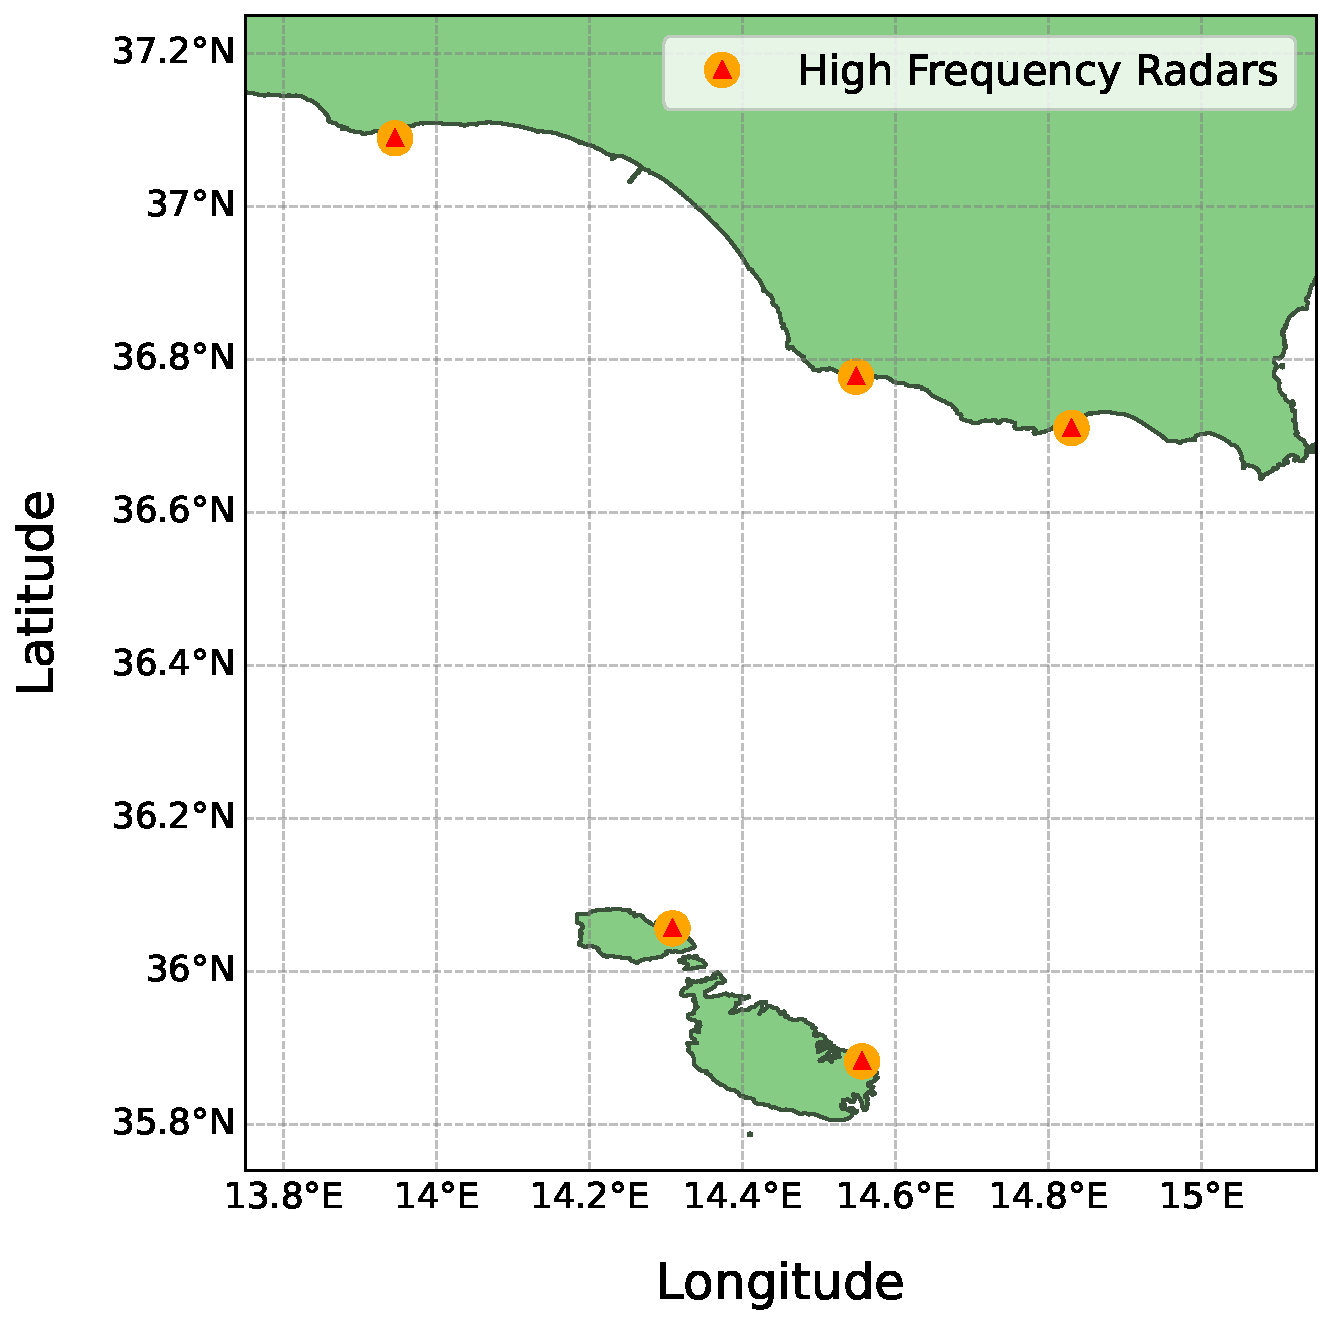
\includegraphics[width=0.5\textwidth, height=0.28\textheight]{radar_locations.pdf}
    \caption[High frequency radars locations.]{-- High frequency radars locations.\label{fig_2.1}}
\end{figure}

The data is composed of several variables including longitude, latitude, and time, coupled with eastern and northern sea current velocities; denoted as \textit{'u'} and \textit{'v'}. The variable \textit{'u'} signifies the east-west current component, indicating the horizontal velocity of surface currents, either eastwards (positive \textit{'u'}) or westwards (negative \textit{'u'}). Similarly, \textit{'v'} represents the north-south current velocity, denoting vertical movement towards the north (positive \textit{'v'}) or south (negative \textit{'v'}). The data's geographical scope is defined within the boundaries of 14.15° to 14.81° longitude and 35.79° to 36.30° latitude. This coverage translates into a grid of 52 latitude points by 43 longitude points, for a total of 180 data points, as detailed in Figure~\ref{fig_2.2}. The dataset is in \acrshort{netcdf} format~\cite{13}, a commonly used format for climate and meteorological data, ensuring compatibility with the Lagrangian Model employed in the simulations.

\begin{figure}[htbp]
    \centering
    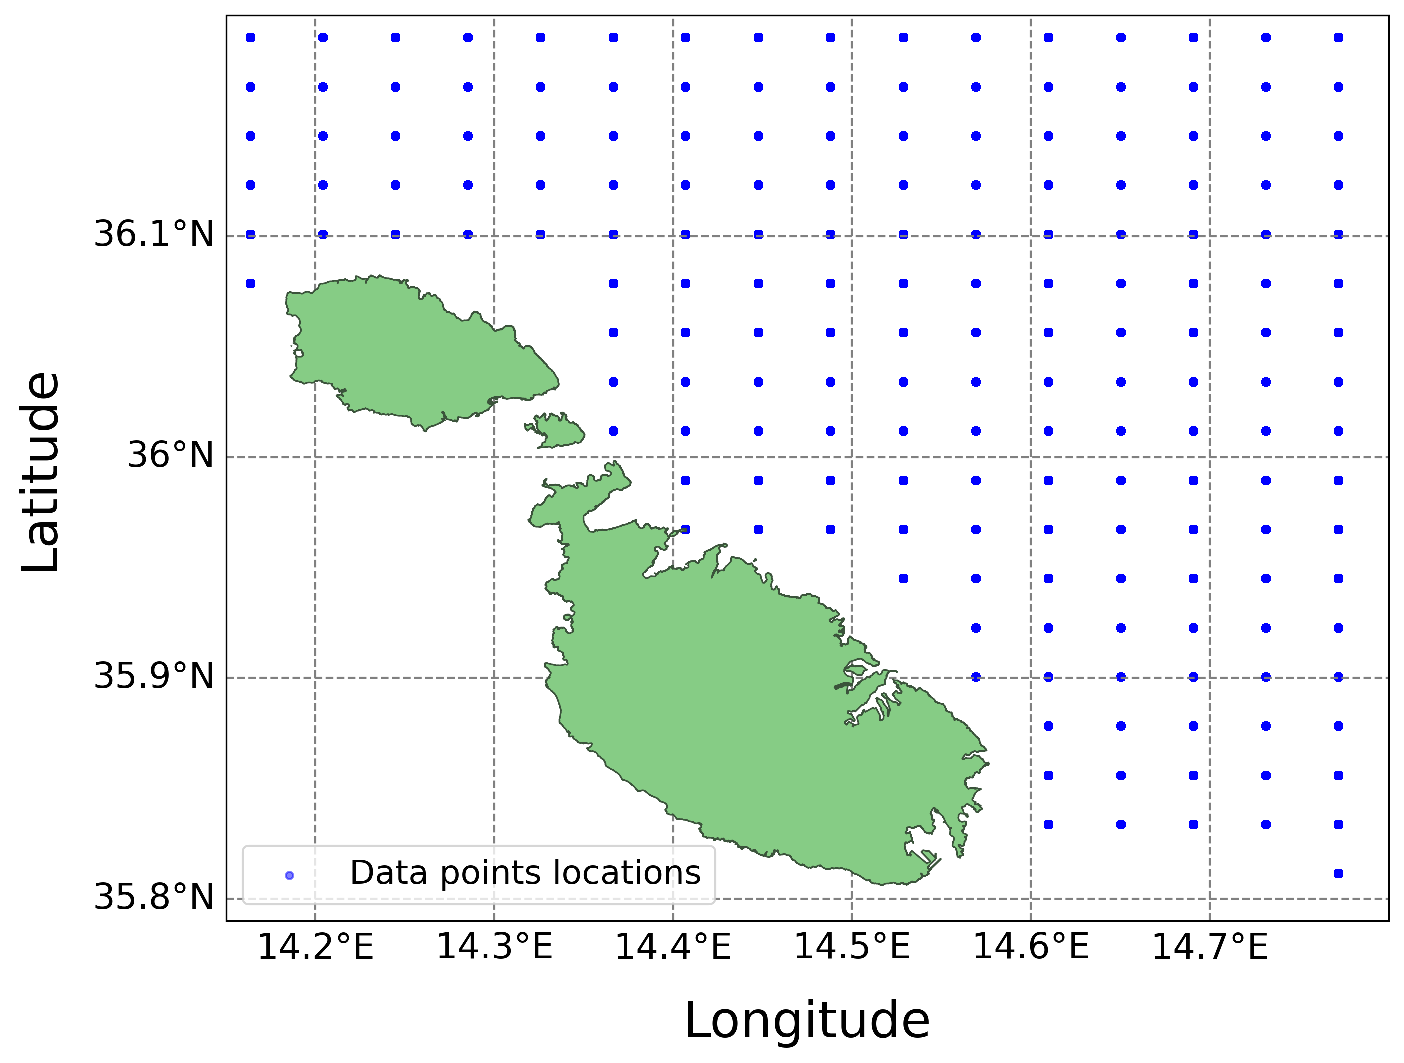
\includegraphics[width=0.48\textwidth,keepaspectratio]{data_locations.pdf}
    \caption[Radar data points locations for dataset.]{-- Radar data points locations for dataset.\label{fig_2.2}}
\end{figure}

This dataset is integral to the project, providing comprehensive environmental parameters essential for the subsequent development of both the physics-based simulations and the Machine Learning models.

\subsection{Physics-Based Lagrangian Model}
\label{subsec:2.1.3}
The practice of tracking ocean surface movements in a Lagrangian framework dates back to the earliest days of oceanography. Early methods involved observing the drift of ships or the paths of specially designed floats to document sea current movement, as outlined by~\cite{14}. The physics-based Lagrangian model~\cite{1} plays a pivotal role in environmental simulations. By offering a dynamic method to trace individual particle trajectories within fluid mediums, the model ensures precise tracking of the particle’s spatio-temporal movement. Its broad applicability spans from localised studies, to global-scale systems. This is evident in its varied applications, such as tracking oil spills diffusion~\cite{15}, mapping floating plastic debris~\cite{16}, simulating jellyfish migrations~\cite{17}, and smoke dispersion~\cite{18}.

The physics-based Lagrangian model~\cite{1} operates by representing particles within a fluid medium, tracking their position and properties as they move with the fluid’s flow. The model calculates the trajectory of each particle by integrating the velocity field of the fluid, which may vary in time and space. This approach enables the simulation of dispersal patterns of particles, such as marine debris, by accounting for both advection and diffusion processes. Advection represents the movement of particles by the flow of the fluid~\cite{19}. Diffusion, on the other hand, models the dispersion of particles through random motion~\cite{19}. This is done by employing techniques such as random walks or Gaussian distributions. This inclusion of randomness enhances the realism of the simulation.

To facilitate these Lagrangian simulations, several Python toolkits like OceanParcels~\cite{20}, PyGnome~\cite{21}, and Flexpart~\cite{22} have been developed. These toolkits enable the customisation and execution of particle tracking simulations, leveraging data on ocean currents, wind fields, and other environmental phenomena. OceanParcels~\cite{20} is distinguished by several features that make it suitable for our project. One of its notable capabilities are custom kernels. These are user-defined functions that allow for tailored simulation scenarios at each time step. Through custom kernels, users can implement complex behaviours and interactions of particles within the fluid, such as particle reflection or response to environmental variables like temperature and wind. Another significant feature is particle initialisation. This feature enables the creation of particles at specific locations, times, and with distinct properties, allowing for more detailed and accurate simulations. 

All these attributes render OceanParcels~\cite{20} as an optimal choice for this project. By integrating these features, this toolkit facilitates the development of comprehensive simulations. This is crucial for understanding and predicting the movement of marine debris, thereby enhancing our strategies for marine conservation and debris management.

\subsection{Time Series Modelling}
\label{subsec:2.1.4}
Time series modelling is a technique used to predict future data points by analysing the trends, cycles, and patterns in a series of data points collected over an interval of time~\cite{23}. The main focus is on analysing historical data to uncover the underlying structure of the data, which can then be used to forecast future trends. This method is particularly powerful for its ability to incorporate the sequence and time dependence within the dataset. By examining how values are interconnected over time, time series models can forecast future values based on the inherent temporal dynamics present in the historical data~\cite{24}. This form of predictive modelling assumes that past patterns shape future behaviours, making it an indispensable tool in a variety of fields ranging from weather forecasting~\cite{25} to stock market predictions~\cite{26}. 

While time series modelling is a powerful tool for forecasting future data, it also possesses some limitations. Time series data often exhibit seasonality and trends, which can complicate the forecasting process~\cite{27}. Outliers, missing sequences of data, and anomalies can also significantly impact the accuracy of forecasting models, requiring careful identification, and handling. The capacity of these models to integrate external influential factors and variables is also somewhat limited, often necessitating the integration of additional features for enhanced predictive accuracy~\cite{28}. Additionally, time series models require significantly more data for training, which can be cumbersome in situations where data is limited~\cite{28}. These challenges highlight the importance of adopting a methodical approach to time series modelling, emphasising the need to carefully consider the specific context and characteristics of the data being analysed when utilising time series models for effective forecasting.

In the context of this \acrshort{fyp}, we harness time series modelling to predict \acrshort{ssc} velocities. Accurate predictions require a detailed analyses of the data sequences to discern patterns that could forecast future predictions. The historical hourly data of surface currents form a time series, which is inherently continuous but sampled at discrete intervals. To address this, deep learning models, a subset of \acrshort{ann}s, are employed due to their proficiency in handling vast amounts of sequential data and their capacity to learn complex temporal patterns~\cite{29}. Through training on past \acrshort{ssc} data, these models are equipped to predict future values.

\subsection{Deep Learning Models}
\label{subsec:2.1.5}
Deep learning is a subset of Machine Learning that harnesses the power of \acrshort{ann}s to interpret and predict data through multiple layers~\cite{30}. Deep learning has revolutionised the way we approach complex problems through its capacity to detect intricate patterns in various types of data~\cite{30}. In the context of this \acrshort{fyp}, deep learning models are pivotal predicting the dynamic and complex patterns of \acrshort{ssc} velocities. By employing models specific to sequential data processing like \acrshort{lstm} and \acrshort{gru} networks, this project aims to accurately predict the dispersion of marine debris around Malta's coastal waters, addressing both the temporal dynamics and spatial complexities inherent in \acrshort{ssc} movements.

\acrshort{lstm} networks are a specialised type of \acrshort{rnn}s. They are designed to address the challenge of learning long-term dependencies, overcoming the limitations faced by traditional \acrshort{rnn}s, notably the vanishing gradient problem~\cite{31}. This challenge inhibits \acrshort{rnn}s from effectively learning and retaining information over long sequences. \acrshort{lstm}s employ a unique architecture, characterised by a system of gates, namely the input, forget, and output gates. These gates collectively decide which information should be stored, discarded, or passed through, based on the relevance to the task at hand~\cite{32}. Memory cells within \acrshort{lstm}s retain information over long intervals, making them adept at managing sequences where understanding past context is crucial for future predictions~\cite{32}. This capability is pivotal for predicting \acrshort{ssc}, as demonstrated in this \acrshort{fyp}. Their ability to remember previous information for extended durations without degradation makes them ideal for capturing the underlying patterns in historical data of \acrshort{ssc}, which is crucial for accurate prediction and subsequent debris dispersion simulations.

 \acrshort{gru} networks are another variant of \acrshort{rnn}s that aim to solve the vanishing gradient problem~\cite{31} but with a more simplified structure compared to \acrshort{lstm}s. \acrshort{gru}s simplify the LSTM model by combining the input and forget gates into a single update gate and merging the cell state and hidden state~\cite{32,33}. This reduction in complexity leads to a model that is faster to train without significantly compromising the model's ability to capture dependencies in a sequence~\cite{32}. In the context of this project, \acrshort{gru}s are employed alongside \acrshort{lstm}s to forecast \acrshort{ssc}. Their efficiency and effectiveness in handling time series data render them adapt at predicting the movements of marine debris, offering a comparative perspective to the \acrshort{lstm}'s performance.

\acrshort{lstm}s and \acrshort{gru}s distinguish themselves primarily through their structure and information processing: \acrshort{lstm}s offer a more detailed gating mechanism that excels in managing long-term dependencies, while \acrshort{gru}s provide a streamlined architecture that enables quicker training without significantly sacrificing performance~\cite{33}. Their inherent capabilities make them exceptionally suited for time series modelling, where understanding and predicting sequential data patterns is crucial~\cite{29}, thereby making them highly applicable to the objectives of this \acrshort{fyp}. It is for these reasons that both models were leveraged in this project, utilising their strengths to predict future \acrshort{ssc} velocities from historical data. Their performances were also compared against one another, aiding in the accurate simulation of marine debris dispersion around Malta's coastal waters.

 \section{Literature Review}
\label{sec:literature_review}
This section outlines the structure of the literature review, which is divided into three distinct subsections, each focusing on a critical aspect of marine debris dispersion and the methodologies employed to predict and simulate it. The first subsection delves into studies that forecast the movement and accumulation of marine debris. The second subsection highlights research that applies Machine Learning techniques to predict \acrshort{ssc}. The final subsection explores the integration between \acrshort{ai} models' predictions and physics-based models. 

\subsection{Prediction of Marine Debris Dispersal}
\label{subsec:2.2.1}
The prediction of marine debris dispersal has significant impact on marine ecosystems. This is why researchers have explored multiple methodologies to understand and forecast the movement and accumulation zones of debris in marine environments. The variation in these approaches reflects the complexity of the problem, encompassing various methods that aim to capture the dynamic nature of marine debris movement. Through the implementation of numerical simulations~\cite{34},~\cite{35}, deep learning techniques~\cite{36}, and advanced simulation tools~\cite{37},~\cite{38}, the field continues to evolve, seeking more accurate and efficient ways to predict debris dispersal patterns.

\subsubsection{Numerical Simulations}
\label{subsubsec:2.2.1.1}

E. van Sebille et al.~\cite{34} focus on the crucial role of numerical simulations in predicting and understanding the dispersion of marine debris. This study utilises a number of numerical simulations that leverage various physical oceanographic phenomena to model the movement of floating marine debris. Central to their approach is the use of extensive datasets, capturing various environmental factors such as the velocity and direction of ocean currents, wind patterns, and wave dynamics. These variables are crucial for determining the dispersal patterns of marine debris.

In~\cite{34}, Eulerian and Lagrangian frameworks are employed. The Eulerian approach models plastics as tracers within a grid, focusing on the interaction between fluid and particle phases, incorporating turbulence through diffusivity parameterisation. Conversely, the Lagrangian framework, preferred for its three-dimensional transport analysis, traces virtual particles using pre-computed velocity data, integrating stochastic terms to reflect the impact of turbulence on dispersion patterns. Both these methods highlight the significant influence of environmental phenomena have on debris movement, especially in nearshore processes. However, accurately simulating coastal dynamics and beaching patterns remains challenging.

Aligning with~\cite{35}, E. van Sebille et al.~\cite{34} highlight the need for enhanced models that better capture surface interactions. Experiments conducted within~\cite{34} and~\cite{35} include the deployment of drifters and buoys equipped with GPS tracking, enabling the researchers to validate their simulation results against real-world data. These findings highlight the importance of integrating numerical simulations with empirical data to refine model accuracy and forecast reliability. Such efforts demonstrate the versatility and efficiency of numerical simulations and ultimately contribute to more effective mitigation and management strategies for marine pollution.

\subsubsection{Deep Learning Techniques}
\label{subsubsec:2.2.1.2}

Computer vision has also emerged as powerful tool in addressing environmental challenges, notably in the management and mitigation of marine debris dispersal, as evidenced in~\cite{36}. These techniques offer approaches to interpret large datasets, enabling more precise and effective solutions to combat marine pollution.

This is illustrated in~\cite{36}, where the authors utilise deep learning and object detection methodologies combined with remote sensing, to automate the identification and classification of marine debris across extensive coastal areas. Specifically, their research targets a stretch of 1900km along the Hawaiian coastline.

The research outlined in~\cite{36} carries out an evaluation of three distinct object detection models, demonstrating an analysis of each model's ability to tackle the complexities involved in detecting marine debris. The research is based on an extensive dataset comprising of 1587 image chips, which together contain 10,703 individual debris labels across various categories. The inclusion of data augmentation techniques further enhances the quality and reliability of the analysis.

Among the key findings, the Single Shot MultiBox Detector (SSD)~\cite{39}, paired with a MobileNet-v2 feature extractor (SS-MN), stands out for its performance by achieving an average precision rate of 72\%. This metric, along with other indicators employed in the~\cite{36}, reinforces the practical viability and efficiency of leveraging deep learning for environmental monitoring. 

The research also acknowledges some challenges and limitations, notably in maximising recall rates to ensure minimal oversight of debris objects. Despite this,~\cite{36} stands as an effective demonstration of how deep learning and computer vision can be strategically deployed to tackle the issue of marine debris dispersal.

\subsubsection{Advanced Simulation Tools}
\label{subsubsec:2.2.1.3}

In our review of methodologies for modelling and simulating surface marine debris dispersal, we have come across numerous studies that employ the OceanParcels toolkit~\cite{20} to tackle issue of simulating marine debris. The work by MS. Yuniarti et al.~\cite{37} provides an insightful analysis of microplastics distribution patterns, which originate from the Seto Inland Sea and extend throughout Japanese waters. OceanParcels~\cite{20} is used to simulate these trajectories. A similar approach is employed in~\cite{38}, where OceanParcels~\cite{20} and the Regional Ocean Modelling System (ROMS) activated with its built-in Lagrangian model, facilitated the tracking of river plume dispersal, highlighting the toolkit's versatility across different marine environments.

Utilising Python-based OceanParcels~\cite{20},~\cite{37} and~\cite{38} delve into the trajectories of particles within marine environments, offering insights into how these different particles navigate through varied marine environments throughout the year. The area simulated by MS. Yuniarti et al.~\cite{37}, spanning latitudes 28° to 55°N and longitudes 120° to 160°E, was strategically selected to optimise the study's focus, similar to the approach in~\cite{38}, where a specific polygon area on the northeast coast of Australia was identified. 

In~\cite{37}, data from the Hybrid Coordinate Ocean Model (HYCOM) provided the necessary current velocities for the simulations, while statistical evaluation employing \acrshort{rmse} validated this data against in-situ observations. The validation process confirmed the suitability of the data for simulation inputs, with \acrshort{rmse} values indicating a close match to observed data, thus improving the accuracy of the simulation results.~\cite{38} used ROMS with a built-in Lagrangian model, incorporating wind fields from global models and recorded river volume discharges, akin to how~\cite{37} utilised HYCOM data to provide current velocities for the simulations.

The findings from~\cite{37} reveal that microplastics dispersion exhibits significant seasonal variations, with distinct pathways and accumulation zones becoming apparent in different seasons. The observed distribution patterns align with those documented within the review of previous studies by MS. Yuniarti et al.~\cite{37}, affirming the reliability of the simulation approach utilised. Furthermore, this enables visualisations that illustrate the dispersal patterns of microplastics, enhancing the spatial and temporal dynamics of marine debris movement.

Both~\cite{37} and~\cite{38} address the challenges associated with tracking large numbers of particles across vast marine areas. These challenges highlight the need for advanced computational resources and methodologies to accurately simulate marine dispersal patterns. The insights from these studies are pivotal in demonstrating the importance of such approaches, paving the way for the development of effective mitigation strategies against marine pollution. This not only advances our understanding of debris trajectories but also establishes a standard for the application of advanced simulation tools like OceanParcels~\cite{20}.

\subsection{Machine Learning Models for Predicting \acrshort{ssc}}
\label{subsec:2.2.2}

As evidenced in~\cite{40}, \acrshort{ssc} are a fundamental phenomenon within ocean hydrodynamics, having a significant influence on various marine processes. Numerous studies have turned to Machine Learning to unravel the intricacies of \acrshort{ssc}, crucial for understanding marine debris dispersion. By leveraging different algorithms, these studies offer new perspectives on marine environmental monitoring, demonstrating the potential of Machine Learning to provide accurate predictions of \acrshort{ssc}.

\subsubsection{Predicting Ocean Currents at Multiple Depths (Single Location)}
\label{subsubsec:2.2.2.1}

Dauji et al.~\cite{41} harness the capabilities of \acrshort{ann}s for the task of predicting ocean currents across multiple depths, not just the sea surface. Ali et al.~\cite{42} employ a similar approach of predicting ocean currents across multiple depths by using \acrshort{lstm} networks. These studies propose time series models to overcome the constraints inherent in numerical models, which necessitate extensive external information, substantial computational resources, and often struggle with noise and gaps in data. 

Both studies highlight the challenge of accurately forecasting ocean currents in different regions.~\cite{41} focuses on two locations within the North Atlantic and North Pacific oceans. This dataset comprises of hourly records of current velocity and direction. These measurements were taken at depths of 18.3m and 460m, representing shallow and deep-water situations. On the other hand, Ali et al.~\cite{42} conduct their study in the Gulf of Mexico. The dataset includes measurements at 50 different depth levels, reaching down to 3000m below the surface, and spans horizontally from 88.5°W to 85°W and 24.65°N to 27°N.

In addressing the challenges posed by the data,~\cite{41} set up a feed-forward back-propagation network \acrshort{ann} architecture, which is recognised for its efficiency. The consideration of additional inputs, specifically currents from lower depths, was explored but ultimately showed no significant improvement to the model's prediction accuracy. In~\cite{42} a deep learning approach was employed using \acrshort{lstm} networks, chosen for their ability to handle long-term dependencies in data. Both studies explored the optimum length of past data segments for input, emphasising the temporal dynamics of sea currents. ~\cite{41} and~\cite{42} encountered and addressed several limitations. One limitation was the initial under-prediction of extreme values in~\cite{41}. This issue was tackled by introducing methods for scaling target extreme values during training. Moreover, due to the high cost and complexity of collecting \acrshort{ssc} data, both studies faced limitations in the availability of long-term observations.

The performance of the \acrshort{ann} models in~\cite{41} was evaluated quantitatively and qualitatively, showing high correlation coefficients and low \acrshort{rmse} and \acrshort{mae} error metrics across various testing durations and prediction intervals. The study also compared the \acrshort{ann} model performance with past works and a random walk model. Notably, the models maintained high performance for currents at both shallow and deep-water layers and were effective across different forecasting durations. The \acrshort{ann} models outperformed traditional forecasting methods, marking a significant improvement in predictive accuracy. The performance of the \acrshort{lstm} models was evaluated using similar error metrics, including \acrshort{rmse}, Peak Signal to Noise Ratio (PSNR), and Structural Similarity (SSIM). 

The studies~\cite{41} and ~\cite{42} validate deep learning models as powerful tools for the real-time prediction of \acrshort{ssc}, demonstrating their success in exceeding the accuracy of traditional forecasting methods.

\subsubsection{Predicting \acrshort{ssc} (Single Location)}
\label{subsubsec:2.2.2.2}

In~\cite{43}, Zulfa et al. investigated the potential of \acrshort{lstm} networks for predicting the velocity and direction of \acrshort{ssc} in Labuan Bajo, Indonesia. Given Labuan Bajo's significance as a pivotal point for trade and tourism, the study aimed to improve maritime navigation and safety through precise forecasts of sea currents.

To conduct this study, Zulfa et al.~\cite{43} utilised a dataset consisting of hourly \acrshort{ssc} velocities collected by the Perak Maritime Meteorology Station II. This dataset is comprised of 24 data points and captures the \acrshort{ssc} velocities at a single geographical point. Before applying any predictive modelling, the data underwent preliminary preprocessing, which included normalisation using the \textit{Min-Max} method. This step was crucial for adjusting the data values to a common scale, thereby facilitating the subsequent training of the predictive model.

The choice of \acrshort{lstm} as the predictive model was driven by its proven effectiveness in handling time-series data, making it particularly suited for forecasting tasks such as predicting \acrshort{ssc} velocities. Zulfa et al.~\cite{43} faced certain limitations, particularly the challenge of applying \acrshort{lstm} to short-term datasets. These models typically excel with long-term data, benefiting from extensive datasets to learn underlying patterns effectively. 

In evaluating the performance of the \acrshort{lstm} model, the Mean Absolute Percentage Error (MAPE) metric was utilised. MAPE measures the accuracy of predicted values compared to actual values. The study achieved notably accurate predictions for the \textit{'u'} and \textit{'v'} components of \acrshort{ssc}, with MAPE values of 14.15\% and 8.43\%, respectively, using a \acrshort{lstm} model configured with 50 hidden layers, a batch size of 32, and a learning rate drop period of 150.

The research concluded that using \acrshort{lstm} networks with specific parameter configurations, serves as a reliable tool for predicting the velocity and direction of \acrshort{ssc}. However,~\cite{43} also suggest that further exploration into methods more suited to short-term data or the inclusion of seasonal variations and tidal factors could enhance predictive accuracy.

Bayindir [40] has a similar approach to~\cite{43}, where the focus is also on using \acrshort{lstm}s to predict \acrshort{ssc}. This choice is motivated by the \acrshort{lstm}'s capability to capture long-term dependencies in sequential data, a common characteristic of \acrshort{ssc}. The study uses a dataset collected by the National Oceanic and Atmospheric Administration (NOAA) in Massachusetts Bay, covering the period from November 2002 to February 2003, with measurements taken at a depth of 23.5m and recorded at intervals every 3 minutes and 44 seconds. This dataset, consisting of the current speed in two directions (\textit{'u'} and \textit{'v'}), undergoes preprocessing to standardise the data, ensuring zero mean and unit variance.

The methodology section stands out by providing a clear and concise explanation of how \acrshort{lstm} networks operate, including their sequence-to-sequence regression capability, which is central to predicting future states of \acrshort{ssc}. Bayindir evaluates the \acrshort{lstm} model's performance by employing the \acrshort{rmse} error metric. This metric offers a direct comparison between the predicted and actual current velocities. 

The results from~\cite{40} demonstrate the \acrshort{lstm} model's ability to make accurate predictions, with significant improvements observed when the model incorporates real-time data updates. Initially, even without these updates, the \acrshort{lstm} model shows a strong capacity for predicting \acrshort{ssc}, suggesting it can make reliable forecasts within a few future time steps. This is highlighted by the model's predictions exhibiting a higher frequency peak compared to the actual observed data, indicating a solid baseline accuracy. However, the research further reveals that when the model is refined with observed values, essentially updating it with real data, the accuracy of predictions markedly increases. This aspect underscores a common hurdle in Machine Learning and deep learning applications, where the quantity and quality of historical data can significantly impact the accuracy of the predicted values.

\subsubsection{Predicting Sea Surface Temperatures (Multiple Locations)}
\label{subsubsec:2.2.2.2}

H.-M. Choi et al.~\cite{44}, develop \acrshort{lstm} networks to predict sea surface temperatures (SSTs) near the Korean Peninsula. The aim is to mitigate the impacts of rising SSTs due to global warming on marine ecosystems and aquaculture. The \acrshort{lstm} models demonstrate promising results in predicting SSTs and identifying high water temperature events with high accuracy for short-term forecasts.

~\cite{44} acknowledges limitations such as decreased prediction accuracy for longer-term forecasts and a reliance solely on SST data without considering other environmental factors. The evaluation of the model's performance was done through metrics like R\textsuperscript{2}, \acrshort{rmse}, MAPE, and F1 score. These metrics collectively assess the model's accuracy and its capability in classifying high water temperature events. The results indicate promising accuracy, particularly for short-term predictions up to four days in advance. However, the model's accuracy decreases for longer prediction windows, highlighting a critical area for improvement.
 
In H.-M. Choi et al.~\cite{44}, the goal of predicting SSTs across a grid of 1519 data points near the Korean Peninsula closely reflects the task we face in forecasting \acrshort{ssc} velocities for various data point locations, which will subsequently be utilised as inputs into a Lagrangian model. By training a predictive model on a 12-year dataset for each data point and then mapping the predictions for subsequent days, it showcases a structured methodology for accurate environmental prediction. This process can be effectively applied to predict conditions across multiple locations in a marine area, paving the way for other applications. 

\subsection{Model Integration with Physics-Based Lagrangian Model}
\label{subsec:2.2.3}

In~\cite{45}, J. Mansui et al. set out to explore the dispersal of floating macro litter across the Mediterranean Sea by employing a two-stage modelling approach to achieve their objective. Initially, they utilised the NEMO Oceanic General Circulation Model, configured specifically for the Mediterranean basin, to simulate the sea state and velocity fields necessary for the drift simulations. This model configuration allows for a fine-scale representation of the region's oceanic conditions, which is crucial for accurate simulation of ocean currents and phenomena. The velocity outputs from this model are taken as daily averages, providing a consistent long-term description of the surface conditions.

Following the generation of these velocity fields, the second stage involves Lagrangian simulations. These simulations use the data from the Oceanic General Circulation Model to simulate the movement of virtual particles that mimic the behaviour of floating macro litter at the sea surface.  To specifically observe the surface transport pathways of the floating macro litter, the method focuses solely on surface movements without considering vertical dynamics or windage. The integration of these two models enables a comprehensive simulation of debris movement and accumulation. 

~\cite{45} produced significant results, demonstrating seasonal and regional variations in floating macro litter distribution across the Mediterranean Sea. These findings were visualised to illustrate accumulation zones, offering a dynamic view of how marine debris disperses over time. The results aligned well with empirical data from previous studies, reinforcing the model's validity and effectiveness. J. Mansui et al. conclude that the integration of Lagrangian simulations with the OGCM offers a powerful framework for predicting marine litter distribution, highlighting its reliability.

In ~\cite{46}, the primary focus is to evaluate floating marine litter within the Northwest Pacific region. This is done by employing an approach that integrates different models with a physics-based Lagrangian model, aiming to enhance the understanding and management of marine litter trajectories.

The methodology employed is noteworthy for the integration of Eulerian models with Lagrangian particle tracking to predict and analyse the behaviour and dispersion patterns of marine litter. Eulerian models provide crucial data on ocean currents and winds by solving fluid dynamics equations on a fixed grid, establishing the environmental values that will be later utilised in the pipeline. Building upon this, the Lagrangian  model simulates the trajectories of individual particles as they navigate through the ocean's dynamic conditions like currents and winds, which are determined by the Eulerian outputs. Through various case studies conducted within the Northwest Pacific region, ~\cite{46} demonstrates the effectiveness of this combined methodology in predicting not only the movement but also the deposition areas of marine litter, providing valuable insights into effective management and mitigation strategies.

~\cite{46} also addresses some challenges inherent in these models. A significant challenge highlighted is that the integration of wind-induced leeway drift poses discrepancies between observed and modelled trajectories, particularly under conditions of strong winds. Overall, The results derived from the applied models are largely successful, providing visual maps and simulations that depict litter trajectories and accumulation zones. These visualisations serve as crucial tools for understanding the impact of physical factors like currents and winds on the distribution of debris.

\section{Summary}
\label{sec:2.3}

This chapter provided a detailed overview for understanding the complex dynamics of marine debris, its ecological impacts, and the methodologies employed to forecast its movements. The background section offered an in-depth understanding of the datasets and outlined the essential components of the project, which included the environmental implications of marine debris and the modelling techniques employed. The Literature Review further expanded on this by examining a number of studies, highlighting advancements and efforts in marine dispersal prediction. This section also aligned the project with various literature, reinforcing the \acrshort{fyp}’s contributions to predictive modelling and the integration of AI models with physics-based models. Collectively, these sections validated the different approaches employed, setting the stage for the subsequent chapters.